\documentclass{bioinfo}
\copyrightyear{2014}
\pubyear{2014}

\begin{document}
\firstpage{1}

\title{Automated HPO-Annotations for newly sequenced proteins by homology inference}
\author{K. Nagaraj$^{1}$, M. Hanumanthappa$^{1}$, O. Tarabai$^{1}$, S. Seitz$^{1}$}
\address{$^{1}$Fakul\"at f\"ur Informatik, Boltzmannstr. 3, 85748 Garching}


\history{Received on 28.02.2014}
\editor{Associate Editor: I12 - Department for Bioinformatics and Computational Biology - Fakult\"at f\"ur Informatik, Boltzmannstr. 3, 85748 Garching}

\maketitle

\begin{abstract}

\section{Motivation:}
Automatic protein function prediction for a novel sequence is an important problem in bioinformatics. Despite the rapid advancement in computational methods used, automatic annotations based on local alignments suffer from several drawbacks \citep{Ori06}. We present a new method for automated Human Phenotype Ontology (HPO) annotation using homology-based inference. Our method uses BLAST tool and a reference database of annotated protein sequences to transfer HPO annotations to an unknown protein based on sequence similarities.
\section{Results:}
Our method achieved an \textit{F-value} of 0.2842 in predicting HPO annotations for unknown protein sequences.
\section{Availability:}
The webinterface for our created prediction-method is available at https://dataminer.informatik.tu-muenchen.de/~omar.tarabai/.

\section{Contact:} \href{assistant@rostlab.org}{assistant@rostlab.org}
\end{abstract}

\section{Introduction}
In the databases many proteins are found for which the sequence is known, but the function is still not determined. With the increasing number of sequences, caused for example by genomic scale projects, traditional experimental approaches have become outpaced. This leads to the need for rapid and reliable functional annotation methods \citep{Rodrigues07}. 

Many different approaches have been taken to annotate protein function using computational methods, including methods based on sequence, expression, interaction and tertiary structure. Despite this taken effort and the following increase in the number and variety of prediction methods, automated annotation remains difficult \citep{Rodrigues07}.

We suggest a new method for automatic HPO term annotation for an unknown protein by input of sequence alone.

\section{Material \& Methods}

Our method mainly relies on using protein sequence similarity as an indicative of functional similarity in order to transfer Human Phenotype Ontology (HPO) annotations from known to unknown protein sequences. Therefore, in order to reach a reasonable prediction, we required a set of HPO annotated protein sequences to use as a reference database. The full HPO-terms database and the gene-to-phenotype mapping were downloaded from \cite{hpodb} on October 4th, 2013. Sequences for the mapped genes were extracted from UniProt \cite{uniprot} database.

We used BLAST 2.2.26 \cite{blastweb} which is a widely-used tool for protein sequence alignment. It takes as input a pre-generated database of reference protein sequences and a target sequence. It employs a heuristic algorithm to search the reference database for sequences that are most similar to the target sequence. Its main output is the top N hits sorted from the most analogous to the least similar protein sequence. Additionally, it outputs a number of other values defining statistics about the degree of similarity discovered, most relevant to our method is "bit score" which is a statistical measure of how good the calculated sequence alignment is \cite{blastscore}.

Our core algorithm takes three parameters as input, \textit{sequence} which is the target protein sequence string, \textit{hits N} which is the number of hits (positive integer) returned by BLAST to be used in the prediction, \textit{threshold T} which is the cut-off value (real number between 0 and 1 inclusive) for the predicted annotation terms according to their confidence parameter.

The algorithm starts by querying BLAST for the top \textit{N} hits for the target sequence against our pre-generated sequence database. For each of the resulting hits, we construct the full HPO tree from the set of HPO annotation terms corresponding to the hit protein, each term in the tree is labelled with the BLAST "bit score". The resulting N trees are merged together into a single prediction tree, the merging is a simple union operation, scores of the same term found in more than one tree are added together in the final prediction tree. All scores are then normalized to the [0,1] range using equation~(\ref{eq:01}) where $S$ is the predicted term score, $S_{min}$ and $S_{max}$ corresponding to the minimum and maximum scores found in the predicted tree respectively. As the final step, the threshold \textit{T} is applied to the predicted tree by removing any terms with a score lower than the threshold. The output of the algorithm is the list of "leaf" terms in the final tree and the corresponding normalized score as the term \textit{confidence} value.

\begin{equation}
S_N = \frac{S - S_{min}}{S_{max} - S_{min}}
\label{eq:01}
\end{equation}

In the case where BLAST does not produce any hits for a given target protein sequence, we construct a "default prediction tree" from the 73 most common HPO terms found in our initial gene-to-phenotype mapping file. 73 is the average number of terms in a HPO annotation tree for all the genes in our reference database.

\section{Results}

An experiment was conducted to arrive at the optimum values for the free parameters \textit{N} and \textit{T} described in the previous section. We ran the algorithm using as input each of the protein sequences that we have HPO annotations for and different values of \textit{N} (5 to 8 inclusive) and \textit{T} (0 to 1 inclusive with a step of 0.1). Since the target sequences used are present in the reference database, we altered the algorithm to query BLAST for the top $N + 1$ hits instead and removed the target protein from the result set. After each run, we compare the resulting prediction tree against the actual HPO tree and calculate the \textit{precision}, \textit{recall} and \textit{F-value} using Equations \ref{eq:02}, \ref{eq:03} and \ref{eq:04} respectively, these values are then averaged over the whole set of target sequences used. Figure \ref{optim} shows the resulting \textit{F-value} for the different values of \textit{N} and \textit{T}. Since \textit{F-value} is considered a compromise between \textit{precision} and \textit{recall}, we use it as an indicative of performance, best results were achieved at \textit{N} = 7 and \textit{T} = 0.2 with an \textit{F-value} = 0.2842.

\begin{equation}
precision = \frac{true positive}{true positive + false positive}
\label{eq:02}
\end{equation}

\begin{equation}
recall = \frac{true positive}{true positive + true negative}
\label{eq:03}
\end{equation}

\begin{equation}
F-value = 2\times\frac{precision \times recall}{precision + recall}
\label{eq:04}
\end{equation}

\begin{figure}[!tpb]
\centerline{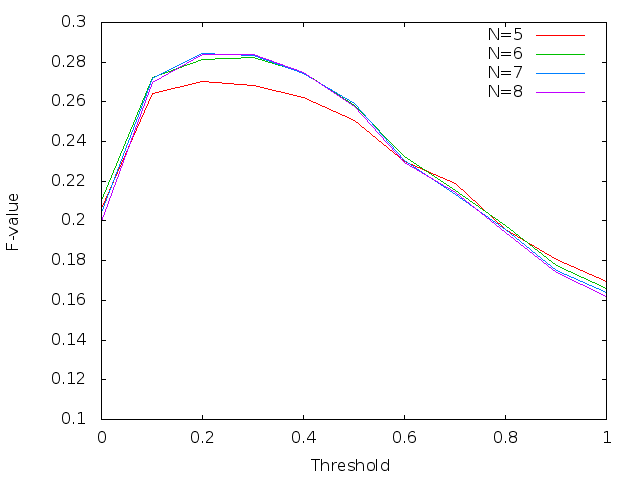
\includegraphics[scale=0.4]{bilder/optim.png}}
\caption{Optimization experiment results}
\label{optim}
\end{figure}

To evaluate the performance effect produced by the "default prediction tree" approach described in the previous section, we reran the experiment without it (i.e. no prediction for target sequences with no hits) and the result was a slight decrease in the F-value curves, particularly the peak performance which was also achieved at \textit{N} = 7 and \textit{T} = 0.2 but with an \textit{F-value} = 0.2736.

Another experiment was was carried out using the 10-fold cross-validation method. The initial database of reference protein sequences was randomly partitioned into ten equal sets, one set was used for testing and the other nine sets were used as the reference database, the experiment was then repeated using a different set for testing and the remaining sets as reference. The partitioning and evaluation were done ten times resulting in a total of one hundred evaluation runs, during which the parameters were fixed at \textit{N} = 7 and \textit{T} = 0.2 which achieved the best performance from the previous experiment. The average \textit{F-value} achieved in this experiment is 0.2790, the slight difference in performance from the preceding experiment could be attributed to the smaller size of the reference database compared to the previous experiment. Figure \ref{precrec} shows the resulting average precision/recall curve.

\begin{figure}[!tpb]
\centerline{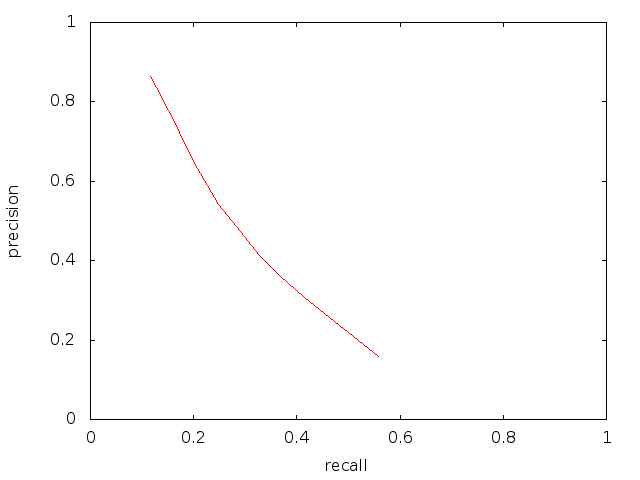
\includegraphics[scale=0.4]{bilder/image-4.png}}
\caption{Precision/recall curve}
\label{precrec}
\end{figure}

Additionally, we performed a comparison between our method and a naive approach in which annotations from the top \textit{N} BLAST hits are transferred directly to the target sequence without any scoring mechanism. We set \textit{N=7} and since there are no scores involved the \textit{T} parameter is irrelevant. The naive approach achieved an \textit{F-value=0.1939}.

\section{Discussion}

Protein function prediction is a difficult problem. Multiple methods are developed to solve different aspects of this problem. Our method relied on homology-based inference of HPO annotation terms for unknown protein sequences, it outperformed the naive approach as shown in the previous section. Nevertheless, we believe there is still room for improvement by evaluating more sophisticated scoring methods.

\section*{Acknowledgement}
Without the great help and guidance by the Rostlab, and every group member there, we wouldn't have been able to succeed in creating our method. Also we would like to thank the Rostlab for letting us access their computers and equipment and Tatyana Goldberg for collecting the data files used.

\begin{thebibliography}{}

\bibitem[BLAST]{blastweb} BLAST: Basic Local Alignment Search Tool. \href{http://blast.ncbi.nlm.nih.gov/Blast.cgi}{http://blast.ncbi.nlm.nih.gov/Blast.cgi}

\bibitem[BLAST score]{blastscore} BLAST Scores and Statistics. \href{http://www.ncbi.nlm.nih.gov/books/NBK21097/\#\_A614\_}{http://www.ncbi.nlm.nih.gov/books/NBK21097/\#\_A614\_}

\bibitem[HPO]{hpodb} Human Phenotype Ontology. \href{http://www.human-phenotype-ontology.org/contao/index.php/downloads.html}{http://www.human-phenotype-ontology.org/contao/index.php/downloads.html}

\bibitem[Ori {\it et~al}. 2006]{Ori06} Sasson, Ori and Kaplan, Noam and Linial, Michal (2006) Functional annotation prediction: All for one and one for all, {\it Protein Science}, {\bf 15}, 1557-1562.

\bibitem[Rodrigues {\it et~al}. 2007]{Rodrigues07} Rodrigues, Ana PC and Grand, Barry J and Godzik, Adam and Friedberg, Iddo (2007) The 2006 Automated Function Prediction Meeting, {\it BMC Bioinformatics}, {\bf 8}, S1. %source: http://www.biomedcentral.com/1471-2105/8/S4/S1

\bibitem[Uniprot]{uniprot} Uniprot: protein sequence and functional information database. \href{http://www.uniprot.org/}{http://www.uniprot.org/}


\end{thebibliography}
\end{document}
